%%%%%%%%%%%%%%%%%%%%%%%%%%%%%%%%%%%%%%%%%%%%%%%%%%%%%%%%%%%%%%%%%%%%%%%%%%%%%%%%
%2345678901234567890123456789012345678901234567890123456789012345678901234567890
%        1         2         3         4         5         6         7         8

\documentclass[letterpaper, 10 pt, conference]{ieeeconf}  % Comment this line out
                                                          % if you need a4paper
%\documentclass[a4paper, 10pt, conference]{ieeeconf}      % Use this line for a4
                                                          % paper





% The following packages can be found on http:\\www.ctan.org
\usepackage{graphics} % for pdf, bitmapped graphics files
\usepackage{epsfig} % for postscript graphics files
\usepackage{mathptmx} % assumes new font selection scheme installed
\usepackage{times} % assumes new font selection scheme installed
\usepackage{amsmath} % assumes amsmath package installed
\usepackage{amssymb}  % assumes amsmath package installed
\usepackage{caption}
\usepackage{subcaption}

\title{\LARGE \bf
  Titel
}

%\author{ \parbox{3 in}{\centering Huibert Kwakernaak*
%         \thanks{*Use the $\backslash$thanks command to put information here}\\
%         Faculty of Electrical Engineering, Mathematics and Computer Science\\
%         University of Twente\\
%         7500 AE Enschede, The Netherlands\\
%         {\tt\small h.kwakernaak@autsubmit.com}}
%         \hspace*{ 0.5 in}
%         \parbox{3 in}{ \centering Pradeep Misra**
%         \thanks{**The footnote marks may be inserted manually}\\
%        Department of Electrical Engineering \\
%         Wright State University\\
%         Dayton, OH 45435, USA\\
%         {\tt\small pmisra@cs.wright.edu}}
%}

\author{Arthur Boetes, Bruno Eijsvoogel, Robert Hauer, Geert Kapteijns
}

\begin{document}


\maketitle
\thispagestyle{empty}
\pagestyle{empty}


%%%%%%%%%%%%%%%%%%%%%%%%%%%%%%%%%%%%%%%%%%%%%%%%%%%%%%%%%%%%%%%%%%%%%%%%%%%%%%%%
\begin{abstract}

Lorem ipsum dolor sit amet, consectetur adipisicing elit, sed do eiusmod tempor
incididunt ut labore et dolore magna aliqua. Ut enim ad minim veniam, quis
nostrud exercitation ullamco laboris nisi ut aliquip ex ea commodo consequat.
Duis aute irure dolor in reprehenderit in voluptate velit esse cillum dolore eu
fugiat nulla pariatur. Excepteur sint occaecat cupidatat non proident, sunt in
culpa qui officia deserunt mollit anim id est laborum.
\end{abstract}


%%%%%%%%%%%%%%%%%%%%%%%%%%%%%%%%%%%%%%%%%%%%%%%%%%%%%%%%%%%%%%%%%%%%%%%%%%%%%%%%
\section{INTRODUCTION}

ipsum dolor sit amet, consectetur adipisicing elit, sed do eiusmod tempor incididunt ut labore et dolore magna aliqua. Ut enim ad minim veniam, quis nostrud exercitation ullamco laboris nisi ut aliquip ex ea commodo consequat. Duis aute irure dolor in reprehenderit in voluptate velit esse cillum dolore eu fugiat nulla pariatur. Excepteur sint occaecat cupidatat non proident, sunt in culpa qui officia deserunt mollit anim id est laborum.

\section{Numerical calculations and results}
The numerical methods used to create the band structure and the butterfly are discussed here.
For this, the matrix \ref{eq:}, is vital.
The arguments of the matrix are $\{k,\phi,\Delta,Q,a\}$.
The mapping to the Hofstadter problem is used where $\Delta = 2t$ and $a = 1$, which is used for all numerical calculations.
The chemical potential is dependent on $Q$ and $a$, see \ref{eq:}.
As has been mentioned before, we look at cases were 
$\frac{Q a}{2 \pi} = \frac{p}{q}$, where $p \leq q$.
For numerical purposes, the matrix is scaled to the hopping parameter $t$, and so all matrix entries are divided by this parameter.
More scaling is achieved by setting $k$ to $qka$.
With this scaling the allowed energies, setting the chemical potential to zero, are between $-4$ and $4$.
For the scaled momenta, $k$, $0 \leq k \leq 2 \pi$.

The matrix has a size of $q$ by $q$ and diagonalizing it yields a spectrum of $q$ eigenvalues which might contain degenerate eigenvalues.
This diagonalization is only possible when all the parameters are fixed, changing any of the parameters might result in a different spectrum.

\subsection{Band structure}
When calculating the band structure, the value of $Q$ is fixed and $k$ is varied. 
The phase $\phi$ can also be varied, but is set to zero for convenience.
Every value of $k$ yields a matrix and in turn every matrix is diagonalized thus yielding an energy spectrum for every $k$.
Grouping these values correctly results in the band structure.

For the different values of 
$\frac{Q a}{2 \pi} \in \{2/3,3/5 \}$ the band structures are plotted in figure \ref{fig:bandstructure}.

\begin{figure}[tbph]
\label{fig:bandstructure}
\begin{subfigure}{.49\linewidth}
\centering
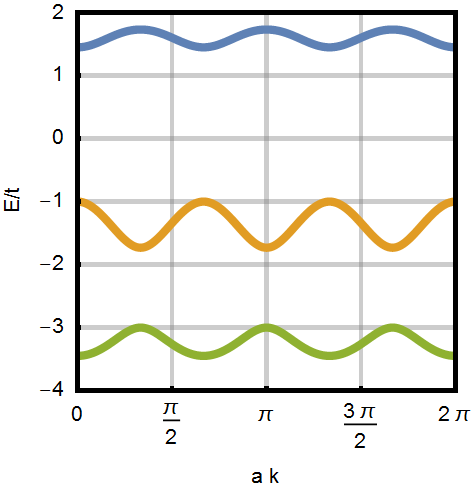
\includegraphics{bandstructure_p=2_q=3.png}
\label{fig:sub1}
\end{subfigure}
\begin{subfigure}{.49\linewidth}
\centering
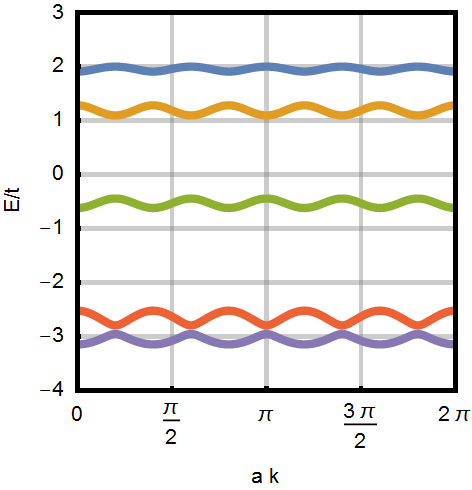
\includegraphics{bandstructure_p=3_q=5.png}
\label{fig:sub2}
\end{subfigure}
\caption{Band structure of the CDW with phase $\phi = 0$.
Left:$p = 2$, $q = 3$ yielding Chern numbers, bottom to top, of -1,1,0.
Right:$p = 3$, $q = 5$ yielding Chern numbers, bottom to top, of 2, -1, 1, -2, 0. }
\end{figure}


\subsection{The CDW butterfly}
Mapping the charge density wave to the Hofstadter problem, and setting the chemical potential to zero, the Hofstadter butterfly is retrieved.
The butterfly can be constructed by fixing $k$ and $\phi$, while varying $Q$.
The relation $\frac{Q a}{2 \pi} = \frac{p}{q}$ must be obeyed however and for numerical calculations an upper limit on $q$ must be made.
The resulting values for $Q$ result from a list of fractions where 
$1 \leq p \leq q$ and all the fractions are reduced to the lowest term, making $p$ and $q$ coprime. 
The requirement of the fractions is that
$0 < \frac{p}{q} \leq 1$.
For a particular value of $\frac{p}{q}$, there are $q$ eigenvalues/bands, and so a list of fractions and energies is obtained.
With every band a Chern number is associated, which can be used to color the butterfly according to the Chern number.



\begin{figure}[tbph]
\label{fig:bandstructure}
\begin{subfigure}{.5\linewidth}
\centering
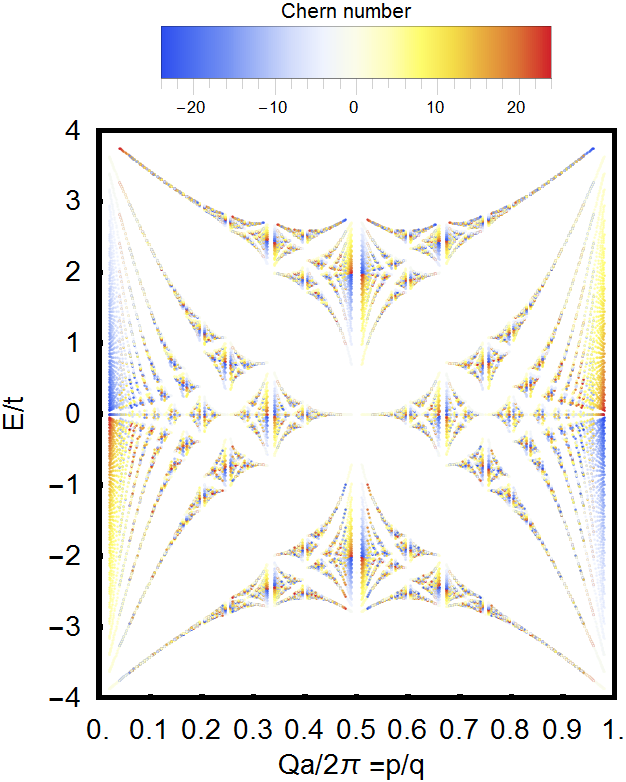
\includegraphics{butterfly50ChernNormalTotal.png}
\label{fig:sub1}
\end{subfigure}
\begin{subfigure}{.1\linewidth}
\centering
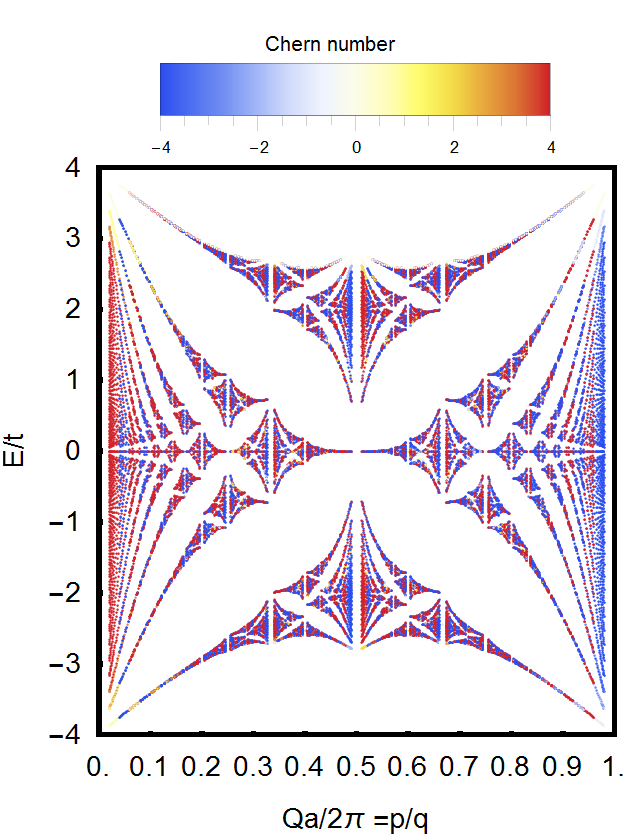
\includegraphics{butterfly50ChernAccuTotal.png}
\label{fig:sub2}
\end{subfigure}
\caption{Allowed energies of the of the CDW Hamiltonian with phase $\phi = 0$ using the method described in this section with a  maximum value of $q = 50$.
Left: The spectrum colored using the Chern numbers.
Right:The energy spectrum where the coloring is done by adding Accumulating the Chern numbers starting at the lowest band and truncating at -4 and 4.}
\end{figure}

\section{One-dimensional charge density waves}

Materials in which the electron density $\rho(x)$ is modulated with a wave of
wavelength $\lambda = \frac{2\pi}{Q}$ are said to contain a charge density wave.
In this paper, we will treat a simple model for a one-dimensional chain of atoms containing such a charge density wave:

$$ H = -t \sum_x (c_x^{\dagger}c_{x+a} + c_x^{\dagger}c_{x-a}) + \sum_x (\mu + \Delta \cos(Qx + \phi))c_x^{\dagger}c_x $$

The first term describes hopping between sites, and the second term contains the chemical potential and the charge density wave.

It is important to notice that if $\lambda = n a$ with $n$ integer and $a$ the lattice spacing, the charge order is said to be commensurate, i.e. the charge modulation is neatly periodic in $n$ lattice sites. If $\lambda$ is not of this form, the charge order is called incommensurate.

After imposing periodic boundary conditions, commensurate charge order is the only option, and the total amount of lattice sites $N$ must equal a multiple of $\lambda$.

To diagonalize $H$, we first apply the canonical Fourier transform:

$$c_x = \frac{1}{\sqrt{N}}\sum_{0 \leq k < \frac{2\pi}{a}}e^{ikx}c_k$$

The hopping term and the chemical potential both give contributions diagonal in $k$. After writing $\cos(Qx + \phi) = \frac{1}{2}(e^{i(Qx + \phi)} + e^{-i(Qx + \phi)}) $, we see that the charge wave in real space gives an off-diagonal contribution in $k$. The resulting Hamiltonian in Fourier space is:

$$ H = \sum_{0 \leq k < \frac{2\pi}{a}} (\frac{1}{2}\epsilon_k c_k^{\dagger}c_k + \Delta_\phi c_k^{\dagger}c_{k+Q} + \text{H.c.}) $$

Where $\epsilon_k = -2t \cos(ka) + \mu $ and $\Delta_\phi = \Delta e^{i\phi}$, i.e. $\Delta$ acquires a phase corresponding to the offset of the charge distribution.

Matrix:
$$
\begin{bmatrix}
\epsilon_k       & \Delta_\phi     & 1      &        & -1     & 2  \\
\Delta_\phi^*    & \epsilon_{k+Q} & \Delta_\phi & \ddots &        & -1 \\
-1               & \Delta_\phi^* & \ddots & \ddots &    \\
   & \ddots & \ddots & \ddots & \ddots & 1  \\
1  &        & \ddots & \ddots & \ddots & -2 \\
-2 & 1      &        & -1     & 2      & 0
\end{bmatrix}
$$

\section{Bruno Stukje}
Let\'s rewrite this Hamiltonian in a nice Matrix form:
\begin{align*}
\hat{H} &= \sum_{0 \leq k < \frac{2\pi}{a}} (\frac{1}{2}\epsilon_k c_k^{\dagger}c_k + \Delta_\phi c_k^{\dagger}c_{k+Q} + \text{H.c.})\\
&=\sum_{0 \leq k < \frac{2\pi}{qa}} \sum_{p=0}^{q-1}  (\frac{1}{2}\epsilon_{k+\frac{2\pi p}{qa}} c_{k+\frac{2\pi p}{qa}}^{\dagger}c_{k+\frac{2\pi p}{qa}} + \Delta_\phi c_{k+\frac{2\pi p}{qa}}^{\dagger}c_{k+\frac{2\pi p}{qa}+Q} + \text{H.c.})\\
\end{align*}


\subsection{Figures and Tables}

Positioning Figures and Tables: Place figures and tables at the top and bottom of columns. Avoid placing them in the middle of columns. Large figures and tables may span across both columns. Figure captions should be below the figures; table heads should appear above the tables. Insert figures and tables after they are cited in the text. Use the abbreviation ÒFig. 1Ó, even at the beginning of a sentence.

\begin{table}[h]
\caption{An Example of a Table}
\label{table_example}
\begin{center}
\begin{tabular}{|c||c|}
\hline
One & Two\\
\hline
Three & Four\\
\hline
\end{tabular}
\end{center}
\end{table}


   \begin{figure}[thpb]
      \centering
      \framebox{\parbox{3in}{We suggest that you use a text box to insert a graphic (which is ideally a 300 dpi TIFF or EPS file, with all fonts embedded) because, in an document, this method is somewhat more stable than directly inserting a picture.
}}
      %\includegraphics[scale=1.0]{figurefile}
      \caption{Inductance of oscillation winding on amorphous
       magnetic core versus DC bias magnetic field}
      \label{figurelabel}
   \end{figure}


Figure Labels: Use 8 point Times New Roman for Figure labels. Use words rather than symbols or abbreviations when writing Figure axis labels to avoid confusing the reader. As an example, write the quantity ÒMagnetizationÓ, or ÒMagnetization, MÓ, not just ÒMÓ. If including units in the label, present them within parentheses. Do not label axes only with units. In the example, write ÒMagnetization (A/m)Ó or ÒMagnetization {A[m(1)]}Ó, not just ÒA/mÓ. Do not label axes with a ratio of quantities and units. For example, write ÒTemperature (K)Ó, not ÒTemperature/K.Ó

\section{CONCLUSIONS}

A conclusion section is not required. Although a conclusion may review the main points of the paper, do not replicate the abstract as the conclusion. A conclusion might elaborate on the importance of the work or suggest applications and extensions.

\addtolength{\textheight}{-12cm}   % This command serves to balance the column lengths
                                  % on the last page of the document manually. It shortens
                                  % the textheight of the last page by a suitable amount.
                                  % This command does not take effect until the next page
                                  % so it should come on the page before the last. Make
                                  % sure that you do not shorten the textheight too much.


\bibliographystyle{plain}
\bibliography{references}


\end{document}